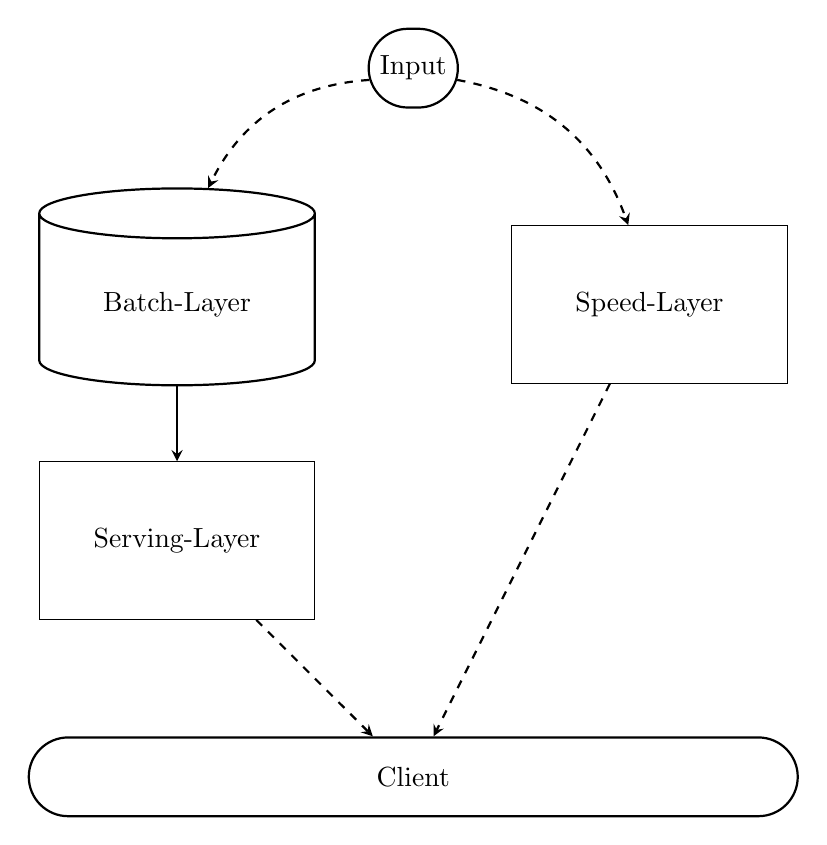
\begin{tikzpicture}[>=stealth]
	\usetikzlibrary{shapes}
	\node (input)			at (3,3) [rounded rectangle, draw, minimum height=1cm,thick] {Input};
	\node (batch)			at (0,0) [cylinder, thick, shape border rotate=90, shape aspect=0.3, draw, minimum height=2.5cm, minimum width=3.5cm] {Batch-Layer};
	\node (serving)		at (0,-3) [rectangle, draw, minimum height=2cm, minimum width=3.5cm,thin] {Serving-Layer};
	\node (speed)			at (6,0) [rectangle, draw, minimum height=2cm, minimum width=3.5cm,thin] {Speed-Layer};
	\node (client)		at (3,-6) [rounded rectangle, draw, minimum height=1cm, minimum width=10cm,thick] {Client};

		\path (input)		edge[->,bend right,dashed,thick] (batch)
		(batch)					edge[->,thick] (serving)
		(serving)				edge[->,dashed,thick] (client)
		(input)					edge[->,bend left,dashed,thick] (speed)
		(speed)					edge[->,dashed,thick] (client);
\end{tikzpicture}
